\section{Aclaración de Conceptos}
En la literatura técnica en español, los términos \textbf{Aprendizaje de Máquina} (traducción literal) y \textbf{Aprendizaje Automático} (traducción formal) se refieren exactamente a la misma disciplina: \textit{Machine Learning}.

Para entender su impacto, el verdadero contraste analítico debe hacerse frente a la automatización clásica, es decir, la \textbf{Programación Tradicional}.

\section{El Duelo: Enfoques y Diferencias}

La diferencia fundamental entre ambos enfoques radica en \textbf{cómo se construyen las reglas} para resolver un problema.

\subsection{1. Programación Tradicional (El enfoque manual)}
En la informática clásica, un humano debe entender el problema a la perfección, deducir la lógica matemática o condicional y escribir las reglas explícitas en código.
\begin{itemize}
    \item \textbf{La Ecuación:} Datos + Reglas dadas por el humano = Respuestas.
    \item \textbf{Limitación:} Si el problema es demasiado complejo o tiene millones de excepciones, es humanamente imposible escribir todas las reglas condicionales (\textit{if/else}).
\end{itemize}

\subsection{2. Aprendizaje Automático (El enfoque basado en datos)}
En el \textit{Machine Learning}, el humano no programa las reglas lógicas. En su lugar, el humano le entrega a la computadora un conjunto masivo de ejemplos (datos y las respuestas correctas de esos datos), y el algoritmo se encarga de descubrir cuáles son las reglas matemáticas que los conectan.
\begin{itemize}
    \item \textbf{La Ecuación:} Datos + Respuestas históricas = Reglas (El Modelo).
    \item \textbf{Ventaja:} Excelente para problemas donde las reglas son ocultas, dinámicas o demasiado complejas (ej. reconocimiento de voz o visión por computadora).
\end{itemize}

\section{Ejemplo de la Vida Real: Filtro Anti-Spam}

Supongamos que queremos crear un sistema que detecte si un correo electrónico es \textit{Spam} o no.

\vspace{0.3cm}
\noindent \textbf{Solución con Programación Tradicional:}
El programador debe escribir reglas estrictas basadas en su intuición:
\begin{verbatim}
SI correo contiene "Gana dinero rápido" ENTONCES Spam = Verdadero
SI remitente es desconocido Y contiene enlace ENTONCES Spam = Verdadero
\end{verbatim}
\textit{Problema:} Los spammers cambian la frase a ``Gana d!nero r4pido'' y el sistema tradicional se rompe, obligando al humano a reescribir el código constantemente.

\vspace{0.3cm}
\noindent \textbf{Solución con Aprendizaje Automático:}
El programador \textbf{no} escribe reglas de palabras. Recolecta 10,000 correos marcados como Spam y 10,000 correos normales. Le pasa todo eso al algoritmo. El modelo analiza la frecuencia de palabras, la estructura y metadatos, y construye su propia red de probabilidades. Si los spammers cambian de táctica, solo hay que reentrenar el modelo con los correos nuevos para que aprenda las nuevas reglas solo.

\vspace{0.5cm}

\section{Representación Gráfica del Paradigma}
El siguiente gráfico ilustra cómo se invierten las entradas y salidas entre ambos enfoques.

\begin{figure}[H]
    \centering
    \shorthandoff{>} % Prevenir errores con babel
    \resizebox{0.95\textwidth}{!}{%
    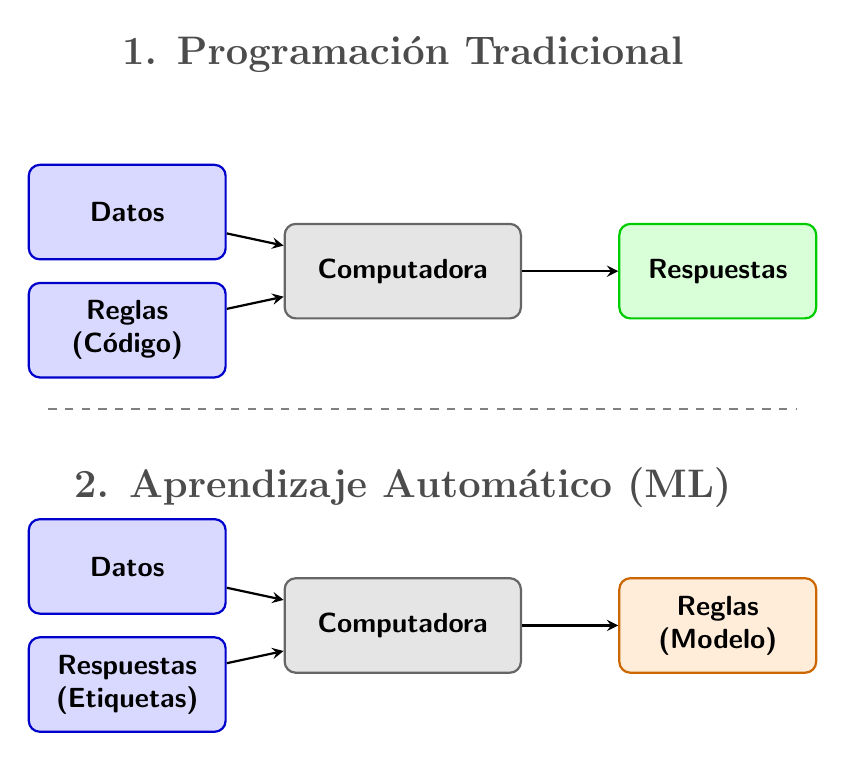
\begin{tikzpicture}[
        % ---> EL FIX ESTÁ AQUÍ: align=center en lugar de text centered <---
        box/.style = {rectangle, rounded corners, draw=black, thick, minimum width=2.5cm, minimum height=1.2cm, align=center, font=\sffamily\bfseries},
        input/.style = {box, fill=blue!15, draw=blue!80!black},
        process/.style = {box, fill=gray!20, draw=gray!80!black, minimum width=3cm},
        output/.style = {box, fill=green!15, draw=green!80!black},
        arrow/.style = {thick, ->, >=stealth}
    ]
    % ================= PARTE SUPERIOR: TRADICIONAL =================
    \node[font=\Large\bfseries, text=black!70] at (3.5, 3) {1. Programación Tradicional};
    
    \node[input] (data1) at (0, 1) {Datos};
    \node[input] (rules1) at (0, -0.5) {Reglas \\ (Código)};
    
    \node[process] (computer1) at (3.5, 0.25) {Computadora};
    
    \node[output] (ans1) at (7.5, 0.25) {Respuestas};

    \draw[arrow] (data1) -- (computer1);
    \draw[arrow] (rules1) -- (computer1);
    \draw[arrow] (computer1) -- (ans1);

    % Línea separadora
    \draw[dashed, thick, gray] (-1, -1.5) -- (8.5, -1.5);

    % ================= PARTE INFERIOR: MACHINE LEARNING =================
    \node[font=\Large\bfseries, text=black!70] at (3.5, -2.5) {2. Aprendizaje Automático (ML)};
    
    \node[input] (data2) at (0, -3.5) {Datos};
    \node[input] (ans2) at (0, -5) {Respuestas \\ (Etiquetas)};
    
    \node[process] (computer2) at (3.5, -4.25) {Computadora};
    
    \node[output, fill=orange!15, draw=orange!80!black] (rules2) at (7.5, -4.25) {Reglas \\ (Modelo)};

    \draw[arrow] (data2) -- (computer2);
    \draw[arrow] (ans2) -- (computer2);
    \draw[arrow] (computer2) -- (rules2);

    \end{tikzpicture}%
    }
    \caption{El cambio fundamental propuesto por el \textit{Machine Learning}: En lugar de programar las reglas para obtener respuestas, proveemos las respuestas para que la máquina descubra las reglas.}
    \label{fig:paradigm_shift}
\end{figure}